\section{Three-model correlation results}
\label{sec:multimodel}
Forward replay and saved correlation analyses are complete for Qwen3.5-35B-A3B, Gemma-4-26B-A4B, and GPT-OSS-20B. Each includes 4,647 attempts from 1,547 source problems on the same six benchmarks, with 100 complete avg@32 groups. All token-limit completions are retained. Completion of class analysis means analysis of available labels, not full annotation coverage. GPT-OSS class tokens occur only in MATH-500 and part of AIME24; the other four benchmarks have no class estimates.
Qwen uses the local deterministic NVFP4 judge described above. Gemma and GPT-OSS use imported Qwen3.8-27B labels, with temperature 1, top-$p$ 0.95, top-$k$ 20, low reasoning effort and a 16,384-token judge budget. Consequently class comparisons also differ in annotation protocol and cohort. Generation uses Qwen GPTQ-Int4, Gemma NVFP4, and GPT-OSS checkpoints respectively; replay settings and selected decoder indices are below. Token counts and absolute position windows are model-specific. Correlations are marginal descriptive associations, not controlled model effects.
\begingroup\scriptsize\setlength{\tabcolsep}{4pt}
\begin{longtable}{@{}llll@{}}
\caption{Replay configuration and mean reasoning length used for position windows.}\label{tab:multi-protocol}\\
\toprule
Model & Replay & Decoder indices & Mean tokens \\
\midrule\endfirsthead
\multicolumn{4}{l}{\textit{Continued from previous page}}\\
\toprule
Model & Replay & Decoder indices & Mean tokens \\
\midrule\endhead
\bottomrule\endfoot
Qwen3.5-35B-A3B & unsloth-4bit & 27, 34, 35, 36, 38, 39 & 12,498.1 \\
Gemma-4-26B-A4B & bnb-4bit & 16, 19, 21, 22, 25, 27, 29 & 10,512.6 \\
GPT-OSS-20B & mxfp4-bf16 & 15, 19, 21, 23 & 5,977.6 \\
\end{longtable}\endgroup

\begingroup\scriptsize\setlength{\tabcolsep}{4pt}
\begin{longtable}{@{}llrrrr@{}}
\caption{All-attempt accuracy and termination by model. Invalid known-gold answers count as incorrect; repeated attempts are not independent problems.}\label{tab:multi-population}\\
\toprule
Model & Dataset & Attempts & Correct & Accuracy & Limit hits \\
\midrule\endfirsthead
\multicolumn{6}{l}{\textit{Continued from previous page}}\\
\toprule
Model & Dataset & Attempts & Correct & Accuracy & Limit hits \\
\midrule\endhead
\bottomrule\endfoot
Qwen3.5-35B-A3B & MATH-500 & 500 & 345 & 0.690 & 17 \\
Qwen3.5-35B-A3B & AIME24 & 960 & 817 & 0.851 & 105 \\
Qwen3.5-35B-A3B & AIME25 & 960 & 773 & 0.805 & 165 \\
Qwen3.5-35B-A3B & Olympiad & 675 & 322 & 0.477 & 89 \\
Qwen3.5-35B-A3B & AMC23 & 1280 & 1238 & 0.967 & 17 \\
Qwen3.5-35B-A3B & Minerva & 272 & 73 & 0.268 & 19 \\
Gemma-4-26B-A4B & MATH-500 & 500 & 353 & 0.706 & 6 \\
Gemma-4-26B-A4B & AIME24 & 960 & 852 & 0.887 & 54 \\
Gemma-4-26B-A4B & AIME25 & 960 & 791 & 0.824 & 103 \\
Gemma-4-26B-A4B & Olympiad & 675 & 349 & 0.517 & 36 \\
Gemma-4-26B-A4B & AMC23 & 1280 & 1249 & 0.976 & 3 \\
Gemma-4-26B-A4B & Minerva & 272 & 82 & 0.301 & 2 \\
GPT-OSS-20B & MATH-500 & 500 & 332 & 0.664 & 4 \\
GPT-OSS-20B & AIME24 & 960 & 681 & 0.709 & 99 \\
GPT-OSS-20B & AIME25 & 960 & 668 & 0.696 & 118 \\
GPT-OSS-20B & Olympiad & 675 & 285 & 0.422 & 34 \\
GPT-OSS-20B & AMC23 & 1280 & 1152 & 0.900 & 6 \\
GPT-OSS-20B & Minerva & 272 & 31 & 0.114 & 0 \\
\end{longtable}\endgroup

\begingroup\scriptsize\setlength{\tabcolsep}{4pt}
\begin{longtable}{@{}llrrrrrr@{}}
\caption{Class token-bearing attempts; classes overlap. Zero coverage implies unavailable estimates.}\label{tab:multi-coverage}\\
\toprule
Model & Class & MATH-500 & AIME24 & AIME25 & Olympiad & AMC23 & Minerva \\
\midrule\endfirsthead
\multicolumn{8}{l}{\textit{Continued from previous page}}\\
\toprule
Model & Class & MATH-500 & AIME24 & AIME25 & Olympiad & AMC23 & Minerva \\
\midrule\endhead
\bottomrule\endfoot
Qwen3.5-35B-A3B & Read & 378 & 30 & 26 & 514 & 27 & 270 \\
Qwen3.5-35B-A3B & Analyze & 424 & 30 & 30 & 619 & 38 & 271 \\
Qwen3.5-35B-A3B & Plan & 407 & 28 & 28 & 507 & 28 & 271 \\
Qwen3.5-35B-A3B & Implement & 477 & 30 & 30 & 667 & 39 & 271 \\
Qwen3.5-35B-A3B & Explore & 260 & 28 & 27 & 474 & 22 & 251 \\
Qwen3.5-35B-A3B & Verify & 400 & 29 & 30 & 617 & 38 & 270 \\
Qwen3.5-35B-A3B & Monitor & 451 & 30 & 29 & 583 & 29 & 272 \\
Gemma-4-26B-A4B & Read & 393 & 28 & 29 & 528 & 34 & 271 \\
Gemma-4-26B-A4B & Analyze & 424 & 30 & 30 & 615 & 40 & 269 \\
Gemma-4-26B-A4B & Plan & 294 & 27 & 28 & 397 & 20 & 244 \\
Gemma-4-26B-A4B & Implement & 478 & 30 & 30 & 656 & 39 & 271 \\
Gemma-4-26B-A4B & Explore & 202 & 26 & 25 & 387 & 20 & 235 \\
Gemma-4-26B-A4B & Verify & 408 & 30 & 30 & 597 & 37 & 261 \\
Gemma-4-26B-A4B & Monitor & 280 & 30 & 29 & 461 & 28 & 251 \\
GPT-OSS-20B & Read & 474 & 68 & 0 & 0 & 0 & 0 \\
GPT-OSS-20B & Analyze & 433 & 68 & 0 & 0 & 0 & 0 \\
GPT-OSS-20B & Plan & 324 & 68 & 0 & 0 & 0 & 0 \\
GPT-OSS-20B & Implement & 500 & 68 & 0 & 0 & 0 & 0 \\
GPT-OSS-20B & Explore & 291 & 44 & 0 & 0 & 0 & 0 \\
GPT-OSS-20B & Verify & 435 & 68 & 0 & 0 & 0 & 0 \\
GPT-OSS-20B & Monitor & 496 & 68 & 0 & 0 & 0 & 0 \\
\end{longtable}\endgroup

\begin{figure}[p]\centering
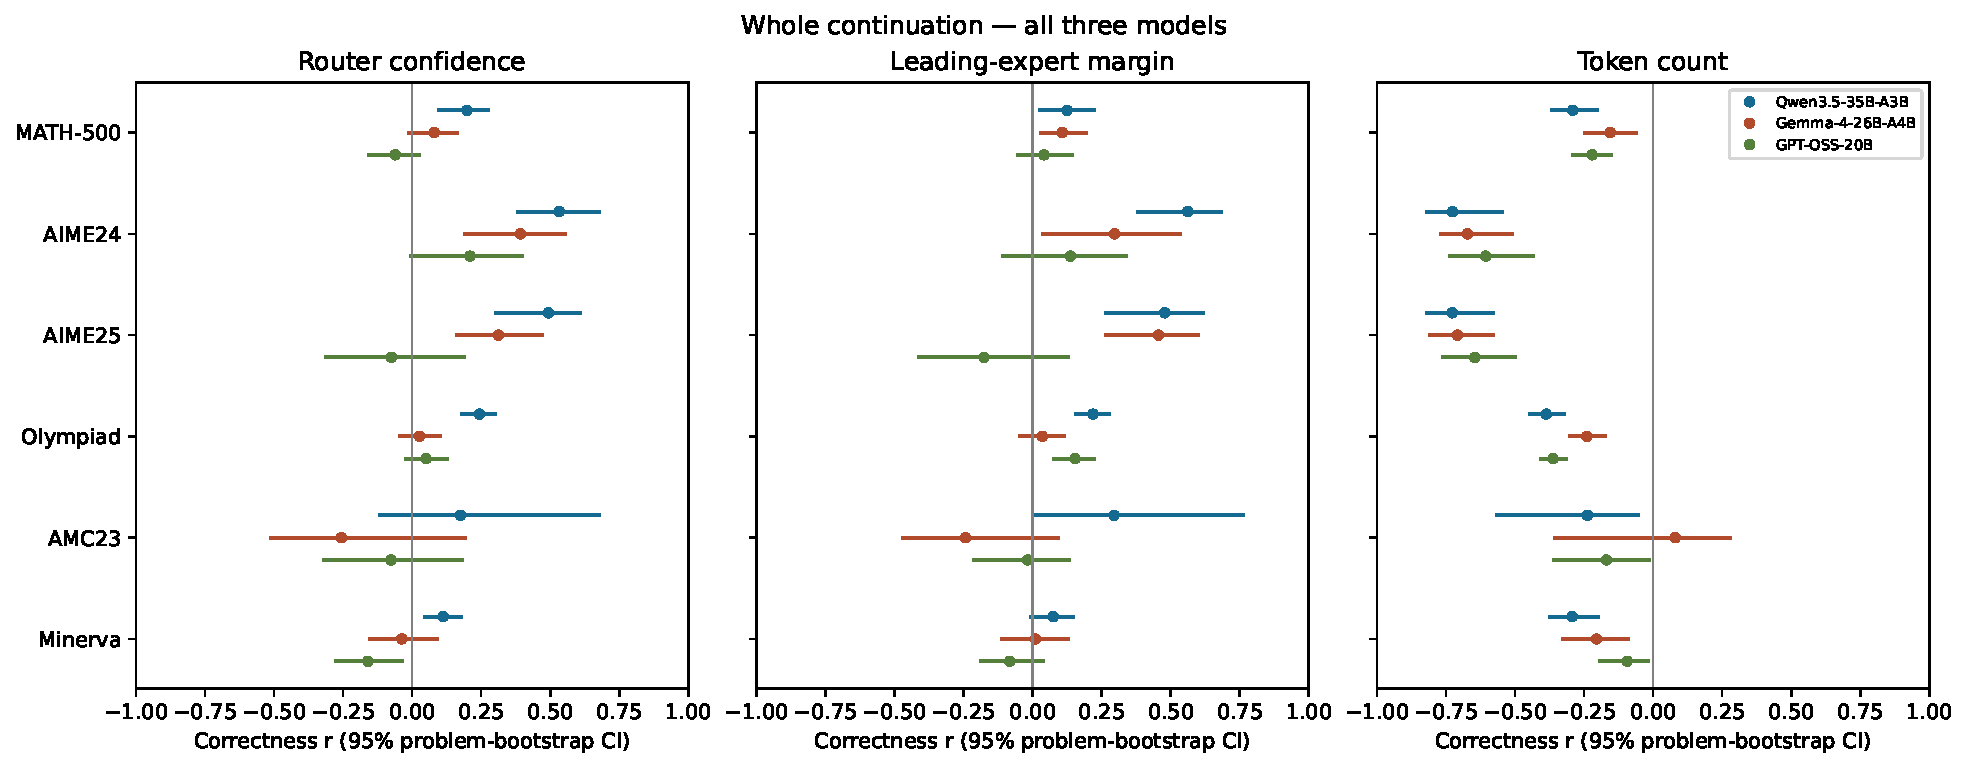
\includegraphics[width=\linewidth]{figures/multimodel_continuation.pdf}
\caption{Whole continuation: saved correctness correlations and pointwise source-problem bootstrap intervals. Overlap or separation of intervals is not a paired test of model differences.}
\Description{Whole continuation: saved correctness correlations and pointwise source-problem bootstrap intervals. Overlap or separation of intervals is not a paired test of model differences.}
\end{figure}

\begin{figure}[p]\centering
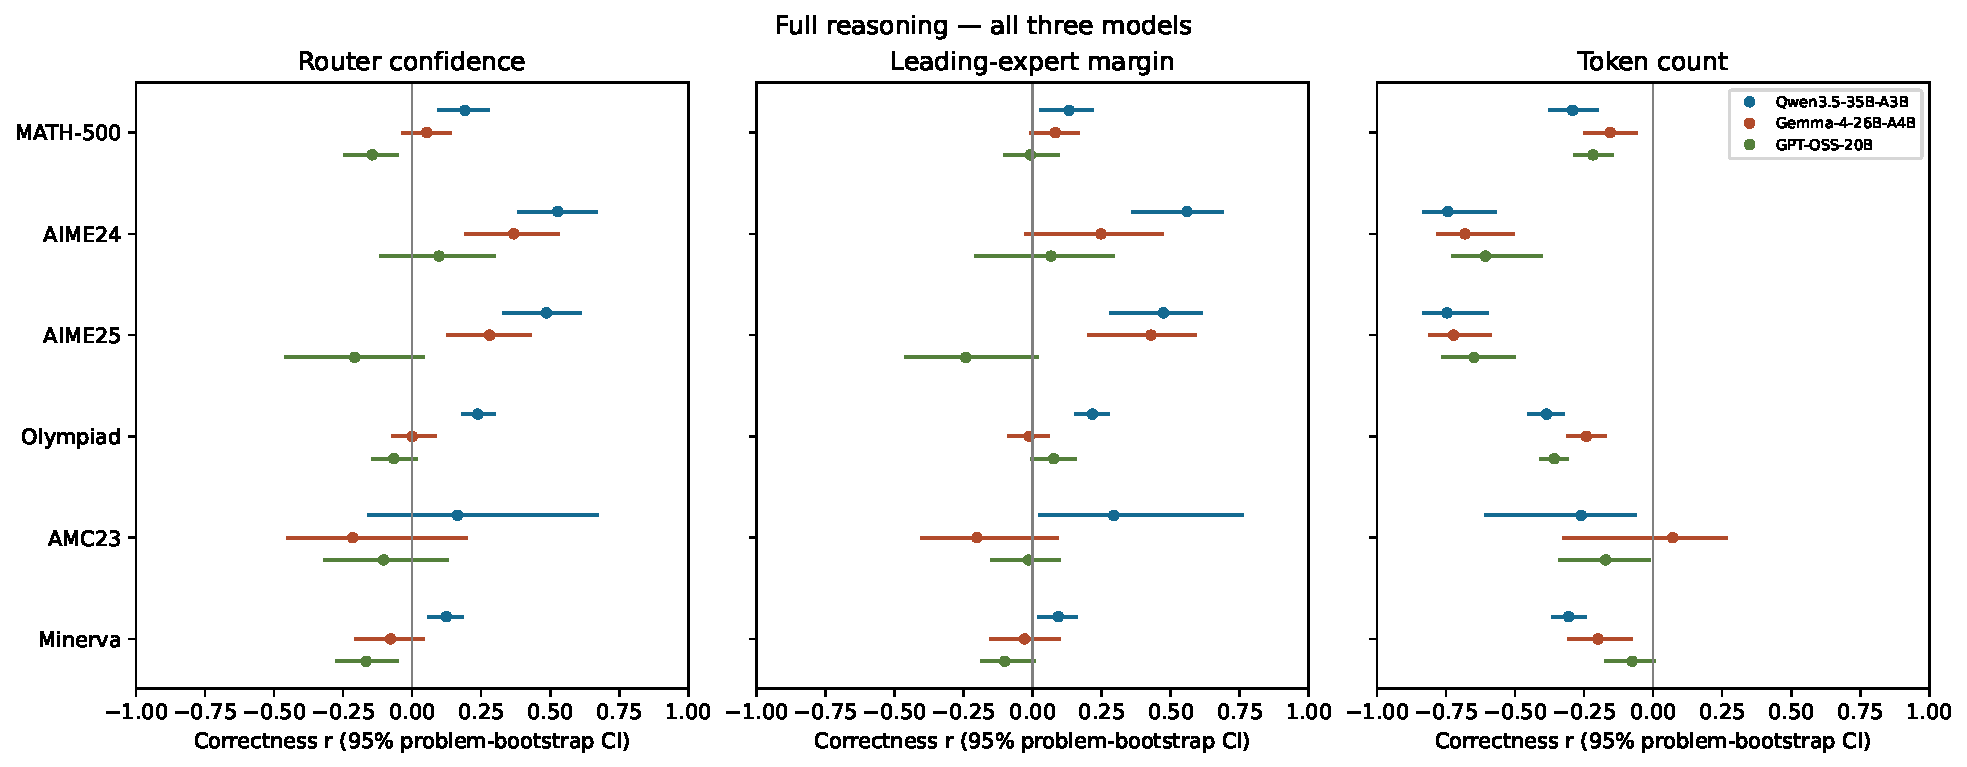
\includegraphics[width=\linewidth]{figures/multimodel_reasoning.pdf}
\caption{Full reasoning: saved correctness correlations and pointwise source-problem bootstrap intervals. Overlap or separation of intervals is not a paired test of model differences.}
\Description{Full reasoning: saved correctness correlations and pointwise source-problem bootstrap intervals. Overlap or separation of intervals is not a paired test of model differences.}
\end{figure}

Across models, confidence--correctness associations do not have a uniform sign. Qwen is positive on all six benchmarks; Gemma is negative on AMC23 and Minerva, and GPT-OSS is negative on MATH-500, AIME25, AMC23, and Minerva. The pointwise intervals in the comparison figures show substantial uncertainty for several of these estimates. Token-count associations are negative except for Gemma on AMC23. These differences motivate model-specific validation rather than assuming that a Qwen-derived routing rule transfers to other models.
\subsection{Qwen3.5-35B-A3B}
\begingroup\scriptsize\setlength{\tabcolsep}{4pt}
\begin{longtable}{@{}lrrrrrr@{}}
\caption{Qwen3.5-35B-A3B: whole-continuation correctness $r$ (finite attempts).}\label{tab:multi-summary-qwen}\\
\toprule
Metric & MATH-500 & AIME24 & AIME25 & Olympiad & AMC23 & Minerva \\
\midrule\endfirsthead
\multicolumn{7}{l}{\textit{Continued from previous page}}\\
\toprule
Metric & MATH-500 & AIME24 & AIME25 & Olympiad & AMC23 & Minerva \\
\midrule\endhead
\bottomrule\endfoot
Token count & $-0.291$ (500) & $-0.726$ (960) & $-0.727$ (960) & $-0.387$ (675) & $-0.238$ (1,280) & $-0.293$ (272) \\
Router confidence & $0.199$ (500) & $0.533$ (960) & $0.493$ (960) & $0.243$ (675) & $0.175$ (1,280) & $0.112$ (272) \\
Leading-expert margin & $0.125$ (500) & $0.562$ (960) & $0.479$ (960) & $0.218$ (675) & $0.295$ (1,280) & $0.075$ (272) \\
Selected probability mass & $0.131$ (500) & $0.175$ (960) & $0.342$ (960) & $0.188$ (675) & $0.097$ (1,280) & $0.082$ (272) \\
Selection-boundary margin & $0.054$ (500) & $-0.035$ (960) & $0.222$ (960) & $0.118$ (675) & $-0.010$ (1,280) & $0.039$ (272) \\
Selected/rest mean gap & $0.131$ (500) & $0.175$ (960) & $0.342$ (960) & $0.188$ (675) & $0.097$ (1,280) & $0.082$ (272) \\
Hidden-state norm & $0.203$ (500) & $-0.018$ (960) & $0.056$ (960) & $0.085$ (675) & $0.550$ (1,280) & $0.083$ (272) \\
Hidden-state step distance & $0.157$ (500) & $0.382$ (960) & $0.404$ (960) & $0.111$ (675) & $0.557$ (1,280) & $0.100$ (272) \\
Hidden/router geometry & $-0.152$ (500) & $-0.058$ (960) & $-0.077$ (960) & $-0.102$ (675) & $-0.229$ (1,280) & $-0.096$ (272) \\
Top-1 switch rate & $-0.071$ (500) & $-0.297$ (960) & $0.141$ (960) & $0.005$ (675) & $-0.160$ (1,280) & $-0.006$ (272) \\
Adjacent selected-set overlap & $0.047$ (500) & $0.022$ (960) & $-0.155$ (960) & $0.016$ (675) & $-0.062$ (1,280) & $-0.010$ (272) \\
\end{longtable}\endgroup

Confidence coefficients in benchmark order are $0.199$, $0.533$, $0.493$, $0.243$, $0.175$, $0.112$.
\begingroup\scriptsize\setlength{\tabcolsep}{4pt}
\begin{longtable}{@{}lrrr@{}}
\caption{Qwen3.5-35B-A3B: problem mean versus avg@32, Spearman $\rho$ (problems).}\label{tab:multi-repeated-qwen}\\
\toprule
Metric & AIME24 & AIME25 & AMC23 \\
\midrule\endfirsthead
\multicolumn{4}{l}{\textit{Continued from previous page}}\\
\toprule
Metric & AIME24 & AIME25 & AMC23 \\
\midrule\endhead
\bottomrule\endfoot
Token count & $-0.861$ (30) & $-0.909$ (30) & $-0.057$ (40) \\
Router confidence & $0.632$ (30) & $0.705$ (30) & $-0.200$ (40) \\
Leading-expert margin & $0.583$ (30) & $0.638$ (30) & $0.190$ (40) \\
Selected probability mass & $-0.112$ (30) & $0.388$ (30) & $-0.215$ (40) \\
Selection-boundary margin & $-0.367$ (30) & $0.135$ (30) & $-0.145$ (40) \\
Selected/rest mean gap & $-0.112$ (30) & $0.388$ (30) & $-0.215$ (40) \\
Hidden-state norm & $-0.384$ (30) & $-0.186$ (30) & $0.484$ (40) \\
Hidden-state step distance & $0.238$ (30) & $0.384$ (30) & $0.504$ (40) \\
Hidden/router geometry & $0.273$ (30) & $0.046$ (30) & $-0.331$ (40) \\
Top-1 switch rate & $-0.381$ (30) & $0.156$ (30) & $0.121$ (40) \\
Adjacent selected-set overlap & $-0.047$ (30) & $-0.196$ (30) & $-0.327$ (40) \\
\end{longtable}\endgroup

\subsection{Gemma-4-26B-A4B}
\begingroup\scriptsize\setlength{\tabcolsep}{4pt}
\begin{longtable}{@{}lrrrrrr@{}}
\caption{Gemma-4-26B-A4B: whole-continuation correctness $r$ (finite attempts).}\label{tab:multi-summary-gemma}\\
\toprule
Metric & MATH-500 & AIME24 & AIME25 & Olympiad & AMC23 & Minerva \\
\midrule\endfirsthead
\multicolumn{7}{l}{\textit{Continued from previous page}}\\
\toprule
Metric & MATH-500 & AIME24 & AIME25 & Olympiad & AMC23 & Minerva \\
\midrule\endhead
\bottomrule\endfoot
Token count & $-0.155$ (500) & $-0.672$ (960) & $-0.709$ (960) & $-0.240$ (675) & $0.080$ (1,280) & $-0.205$ (272) \\
Router confidence & $0.080$ (500) & $0.392$ (960) & $0.313$ (960) & $0.027$ (675) & $-0.256$ (1,280) & $-0.037$ (272) \\
Leading-expert margin & $0.108$ (500) & $0.297$ (960) & $0.456$ (960) & $0.036$ (675) & $-0.243$ (1,280) & $0.010$ (272) \\
Selected probability mass & $0.072$ (500) & $0.375$ (960) & $0.259$ (960) & $0.009$ (675) & $-0.217$ (1,280) & $-0.061$ (272) \\
Selection-boundary margin & $-0.027$ (500) & $0.261$ (960) & $0.068$ (960) & $-0.043$ (675) & $-0.128$ (1,280) & $-0.028$ (272) \\
Selected/rest mean gap & $0.072$ (500) & $0.375$ (960) & $0.259$ (960) & $0.009$ (675) & $-0.217$ (1,280) & $-0.061$ (272) \\
Hidden-state norm & $0.036$ (500) & $0.161$ (960) & $0.007$ (960) & $-0.005$ (675) & $0.104$ (1,280) & $0.003$ (272) \\
Hidden-state step distance & $0.010$ (500) & $0.272$ (960) & $0.440$ (960) & $0.001$ (675) & $-0.141$ (1,280) & $0.059$ (272) \\
Hidden/router geometry & $-0.068$ (500) & $0.020$ (960) & $0.000$ (960) & $-0.019$ (675) & $-0.043$ (1,280) & $-0.076$ (272) \\
Top-1 switch rate & $0.052$ (500) & $-0.133$ (960) & $0.222$ (960) & $0.048$ (675) & $-0.116$ (1,280) & $0.100$ (272) \\
Adjacent selected-set overlap & $-0.021$ (500) & $0.129$ (960) & $-0.244$ (960) & $-0.049$ (675) & $0.038$ (1,280) & $-0.117$ (272) \\
\end{longtable}\endgroup

Confidence coefficients in benchmark order are $0.080$, $0.392$, $0.313$, $0.027$, $-0.256$, $-0.037$.
\begingroup\scriptsize\setlength{\tabcolsep}{4pt}
\begin{longtable}{@{}lrrr@{}}
\caption{Gemma-4-26B-A4B: problem mean versus avg@32, Spearman $\rho$ (problems).}\label{tab:multi-repeated-gemma}\\
\toprule
Metric & AIME24 & AIME25 & AMC23 \\
\midrule\endfirsthead
\multicolumn{4}{l}{\textit{Continued from previous page}}\\
\toprule
Metric & AIME24 & AIME25 & AMC23 \\
\midrule\endhead
\bottomrule\endfoot
Token count & $-0.744$ (30) & $-0.917$ (30) & $-0.099$ (40) \\
Router confidence & $0.473$ (30) & $0.468$ (30) & $0.071$ (40) \\
Leading-expert margin & $0.586$ (30) & $0.777$ (30) & $0.191$ (40) \\
Selected probability mass & $0.416$ (30) & $0.403$ (30) & $0.027$ (40) \\
Selection-boundary margin & $0.345$ (30) & $0.182$ (30) & $-0.063$ (40) \\
Selected/rest mean gap & $0.416$ (30) & $0.403$ (30) & $0.027$ (40) \\
Hidden-state norm & $0.026$ (30) & $-0.042$ (30) & $-0.060$ (40) \\
Hidden-state step distance & $0.410$ (30) & $0.547$ (30) & $-0.063$ (40) \\
Hidden/router geometry & $0.300$ (30) & $0.042$ (30) & $-0.004$ (40) \\
Top-1 switch rate & $-0.367$ (30) & $0.285$ (30) & $-0.215$ (40) \\
Adjacent selected-set overlap & $0.213$ (30) & $-0.321$ (30) & $0.059$ (40) \\
\end{longtable}\endgroup

\subsection{GPT-OSS-20B}
\begingroup\scriptsize\setlength{\tabcolsep}{4pt}
\begin{longtable}{@{}lrrrrrr@{}}
\caption{GPT-OSS-20B: whole-continuation correctness $r$ (finite attempts).}\label{tab:multi-summary-gptoss}\\
\toprule
Metric & MATH-500 & AIME24 & AIME25 & Olympiad & AMC23 & Minerva \\
\midrule\endfirsthead
\multicolumn{7}{l}{\textit{Continued from previous page}}\\
\toprule
Metric & MATH-500 & AIME24 & AIME25 & Olympiad & AMC23 & Minerva \\
\midrule\endhead
\bottomrule\endfoot
Token count & $-0.221$ (500) & $-0.606$ (960) & $-0.646$ (960) & $-0.362$ (675) & $-0.169$ (1,280) & $-0.094$ (272) \\
Router confidence & $-0.061$ (500) & $0.210$ (960) & $-0.075$ (960) & $0.051$ (675) & $-0.077$ (1,280) & $-0.160$ (272) \\
Leading-expert margin & $0.041$ (500) & $0.137$ (960) & $-0.176$ (960) & $0.154$ (675) & $-0.018$ (1,280) & $-0.082$ (272) \\
Selected probability mass & $-0.052$ (500) & $0.128$ (960) & $-0.102$ (960) & $0.089$ (675) & $-0.033$ (1,280) & $-0.166$ (272) \\
Selection-boundary margin & $-0.036$ (500) & $-0.218$ (960) & $-0.091$ (960) & $-0.064$ (675) & $-0.005$ (1,280) & $-0.032$ (272) \\
Selected/rest mean gap & $-0.052$ (500) & $0.128$ (960) & $-0.102$ (960) & $0.089$ (675) & $-0.033$ (1,280) & $-0.166$ (272) \\
Hidden-state norm & $0.192$ (500) & $0.494$ (960) & $0.366$ (960) & $0.329$ (675) & $0.049$ (1,280) & $-0.006$ (272) \\
Hidden-state step distance & $-0.150$ (500) & $-0.186$ (960) & $-0.404$ (960) & $-0.210$ (675) & $-0.094$ (1,280) & $0.045$ (272) \\
Hidden/router geometry & $0.002$ (500) & $-0.239$ (960) & $-0.311$ (960) & $-0.076$ (675) & $-0.027$ (1,280) & $0.053$ (272) \\
Top-1 switch rate & $0.181$ (500) & $0.149$ (960) & $0.376$ (960) & $0.110$ (675) & $-0.006$ (1,280) & $0.331$ (272) \\
Adjacent selected-set overlap & $-0.198$ (500) & $-0.068$ (960) & $-0.278$ (960) & $-0.143$ (675) & $-0.052$ (1,280) & $-0.317$ (272) \\
\end{longtable}\endgroup

Confidence coefficients in benchmark order are $-0.061$, $0.210$, $-0.075$, $0.051$, $-0.077$, $-0.160$.
\begingroup\scriptsize\setlength{\tabcolsep}{4pt}
\begin{longtable}{@{}lrrr@{}}
\caption{GPT-OSS-20B: problem mean versus avg@32, Spearman $\rho$ (problems).}\label{tab:multi-repeated-gptoss}\\
\toprule
Metric & AIME24 & AIME25 & AMC23 \\
\midrule\endfirsthead
\multicolumn{4}{l}{\textit{Continued from previous page}}\\
\toprule
Metric & AIME24 & AIME25 & AMC23 \\
\midrule\endhead
\bottomrule\endfoot
Token count & $-0.889$ (30) & $-0.908$ (30) & $-0.338$ (40) \\
Router confidence & $0.337$ (30) & $0.104$ (30) & $0.186$ (40) \\
Leading-expert margin & $0.248$ (30) & $-0.028$ (30) & $0.262$ (40) \\
Selected probability mass & $0.186$ (30) & $0.046$ (30) & $0.272$ (40) \\
Selection-boundary margin & $-0.356$ (30) & $-0.273$ (30) & $0.060$ (40) \\
Selected/rest mean gap & $0.186$ (30) & $0.046$ (30) & $0.272$ (40) \\
Hidden-state norm & $0.733$ (30) & $0.655$ (30) & $0.338$ (40) \\
Hidden-state step distance & $-0.341$ (30) & $-0.655$ (30) & $-0.289$ (40) \\
Hidden/router geometry & $-0.658$ (30) & $-0.474$ (30) & $-0.177$ (40) \\
Top-1 switch rate & $0.162$ (30) & $0.546$ (30) & $-0.151$ (40) \\
Adjacent selected-set overlap & $-0.029$ (30) & $-0.340$ (30) & $-0.089$ (40) \\
\end{longtable}\endgroup

Aggregate correctness and metric-pair coefficients were independently recomputed from saved CSVs in all 60 model/scope combinations; repeated-problem mean correlations and within-problem contrasts were also checked. This validates numerical consistency, not judge accuracy or replay fidelity. Audit counts and numerical errors are saved in \path{report/multimodel_correlation_audit.json}; input SHA-256 hashes are in \path{report/multimodel_correlation_sources.json}. The appended atlases include every Gemma and GPT-OSS scope, including empty class panels. Full correctness tables are available in \path{report/multimodel_correlation_tables.tex}.
\begin{figure}[p]\centering
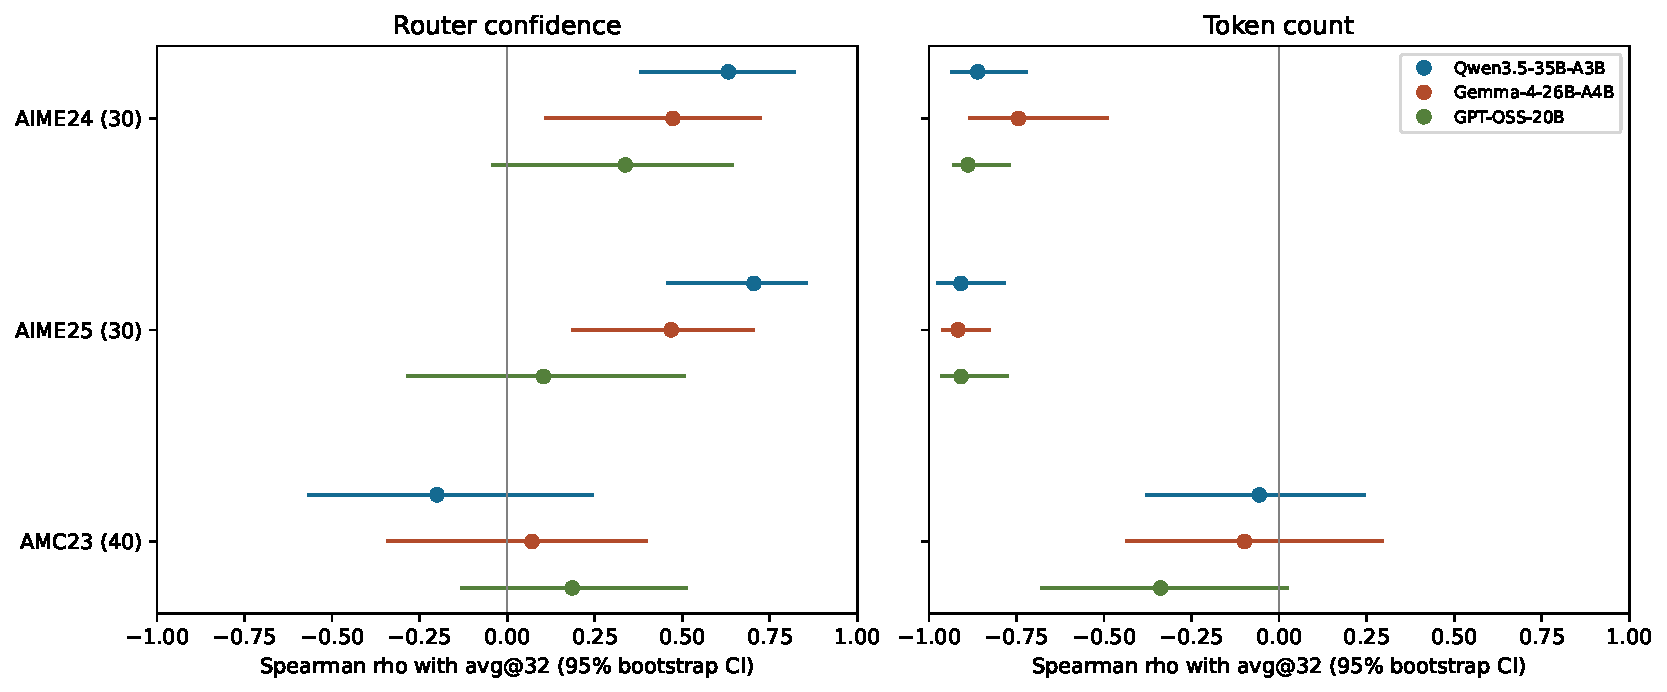
\includegraphics[width=\linewidth]{figures/multimodel_repeated.pdf}
\caption{All models: whole-continuation problem means versus avg@32, with saved pointwise problem-bootstrap intervals. All 32 attempts enter each problem mean.}
\Description{All models: whole-continuation problem means versus avg@32, with saved pointwise problem-bootstrap intervals. All 32 attempts enter each problem mean.}
\end{figure}

\begin{figure}[p]\centering
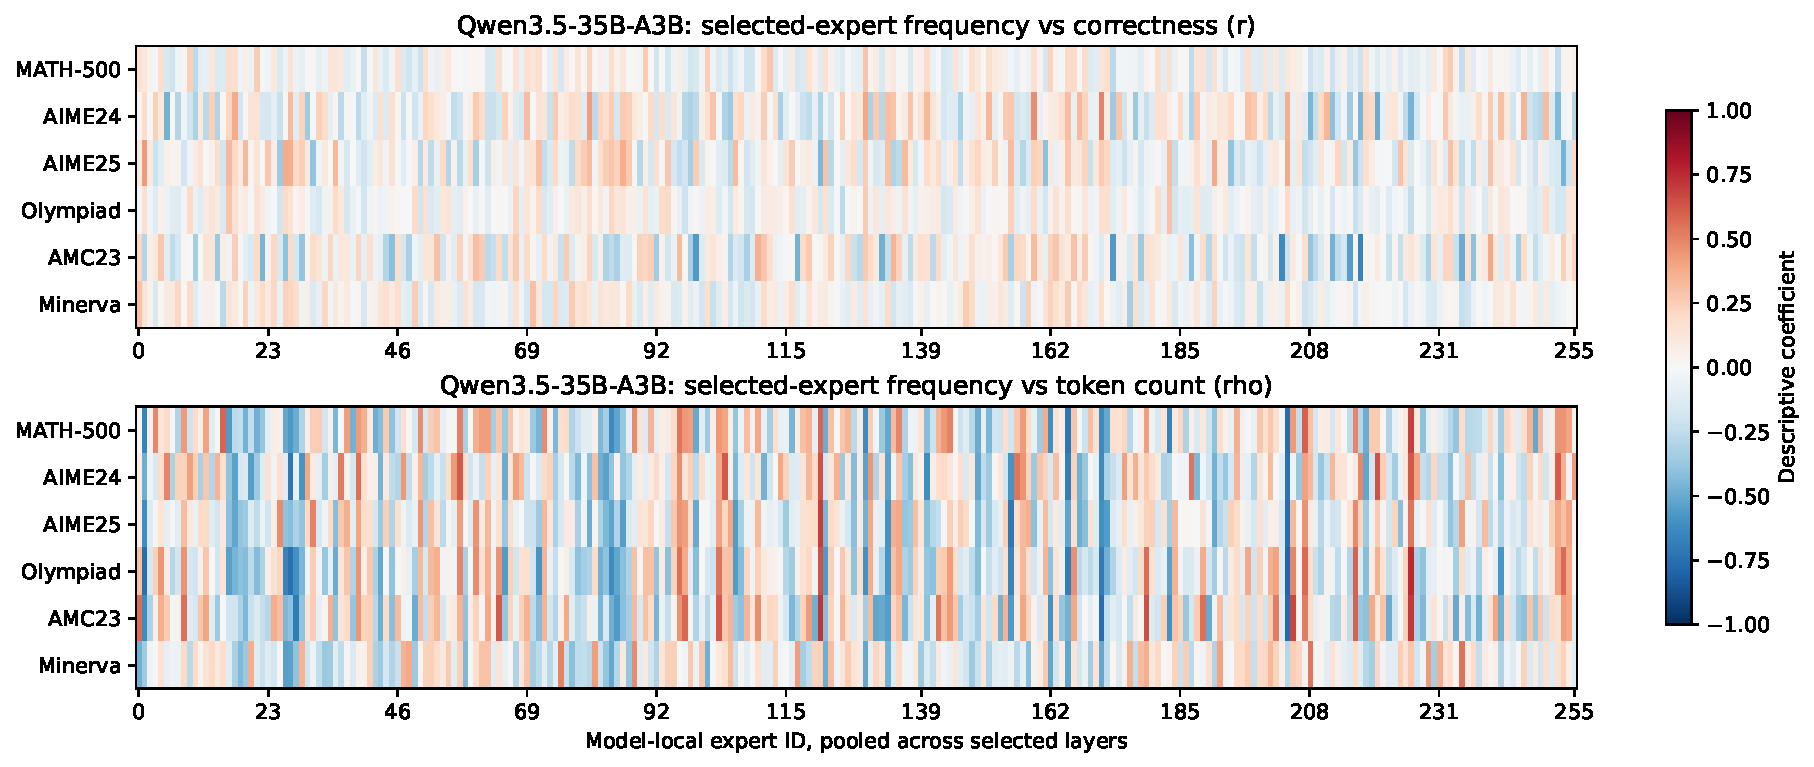
\includegraphics[width=\linewidth]{figures/qwen_multimodel_experts.pdf}
\caption{Qwen3.5-35B-A3B: selected-pool expert frequency correlations with correctness and token count. IDs are model-local and pooled across selected layers; they do not identify matching experts across models. Missing coefficients are blank.}
\Description{Qwen3.5-35B-A3B: selected-pool expert frequency correlations with correctness and token count. IDs are model-local and pooled across selected layers; they do not identify matching experts across models. Missing coefficients are blank.}
\end{figure}

\begin{figure}[p]\centering
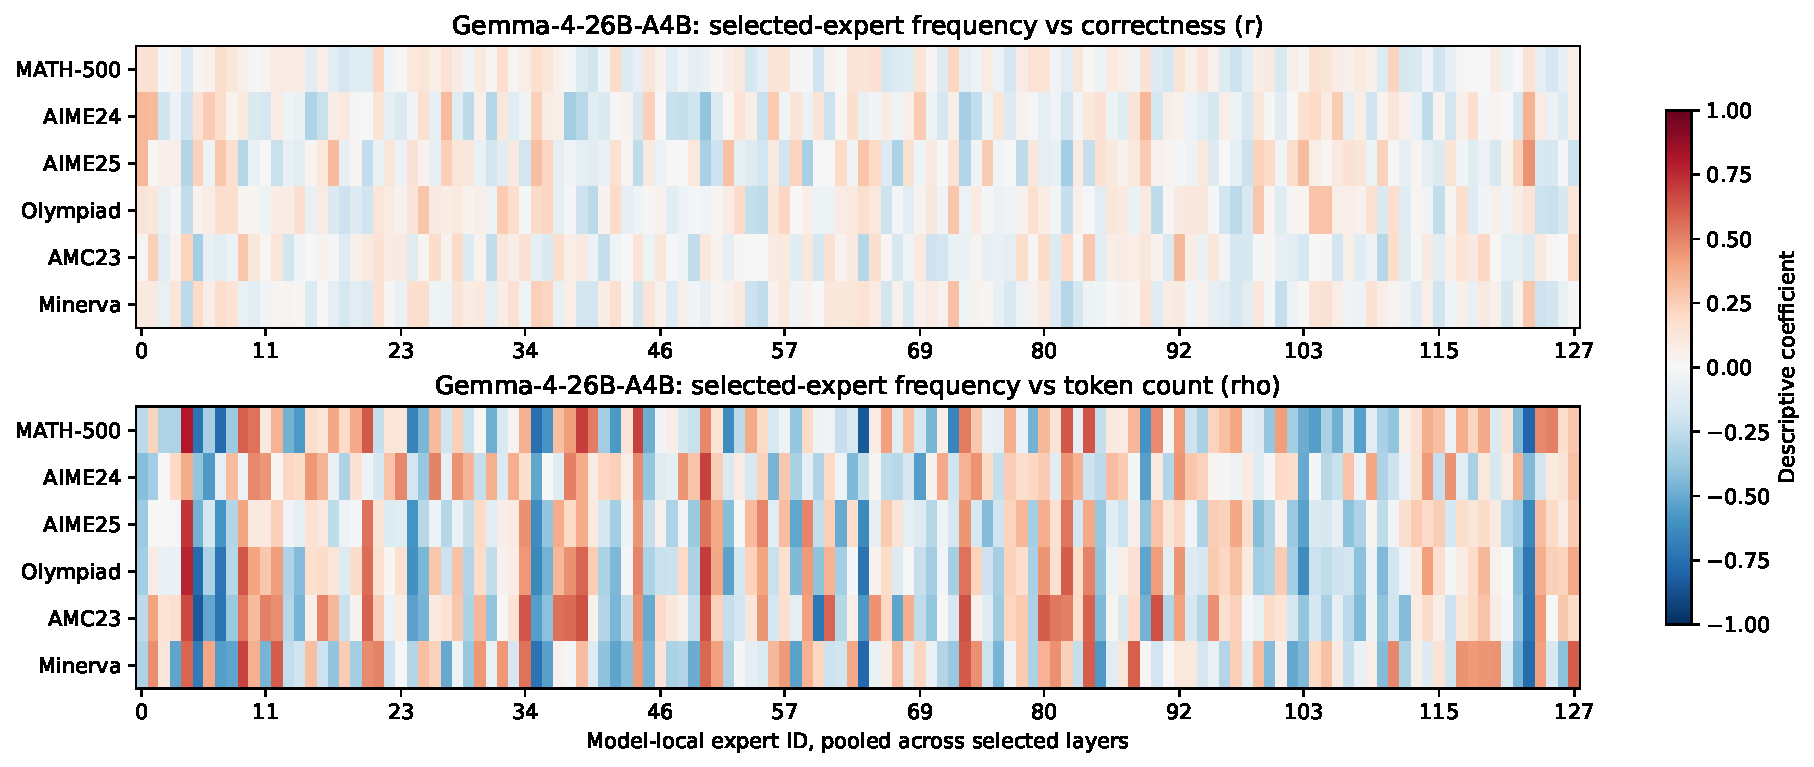
\includegraphics[width=\linewidth]{figures/gemma_multimodel_experts.pdf}
\caption{Gemma-4-26B-A4B: selected-pool expert frequency correlations with correctness and token count. IDs are model-local and pooled across selected layers; they do not identify matching experts across models. Missing coefficients are blank.}
\Description{Gemma-4-26B-A4B: selected-pool expert frequency correlations with correctness and token count. IDs are model-local and pooled across selected layers; they do not identify matching experts across models. Missing coefficients are blank.}
\end{figure}

\begin{figure}[p]\centering
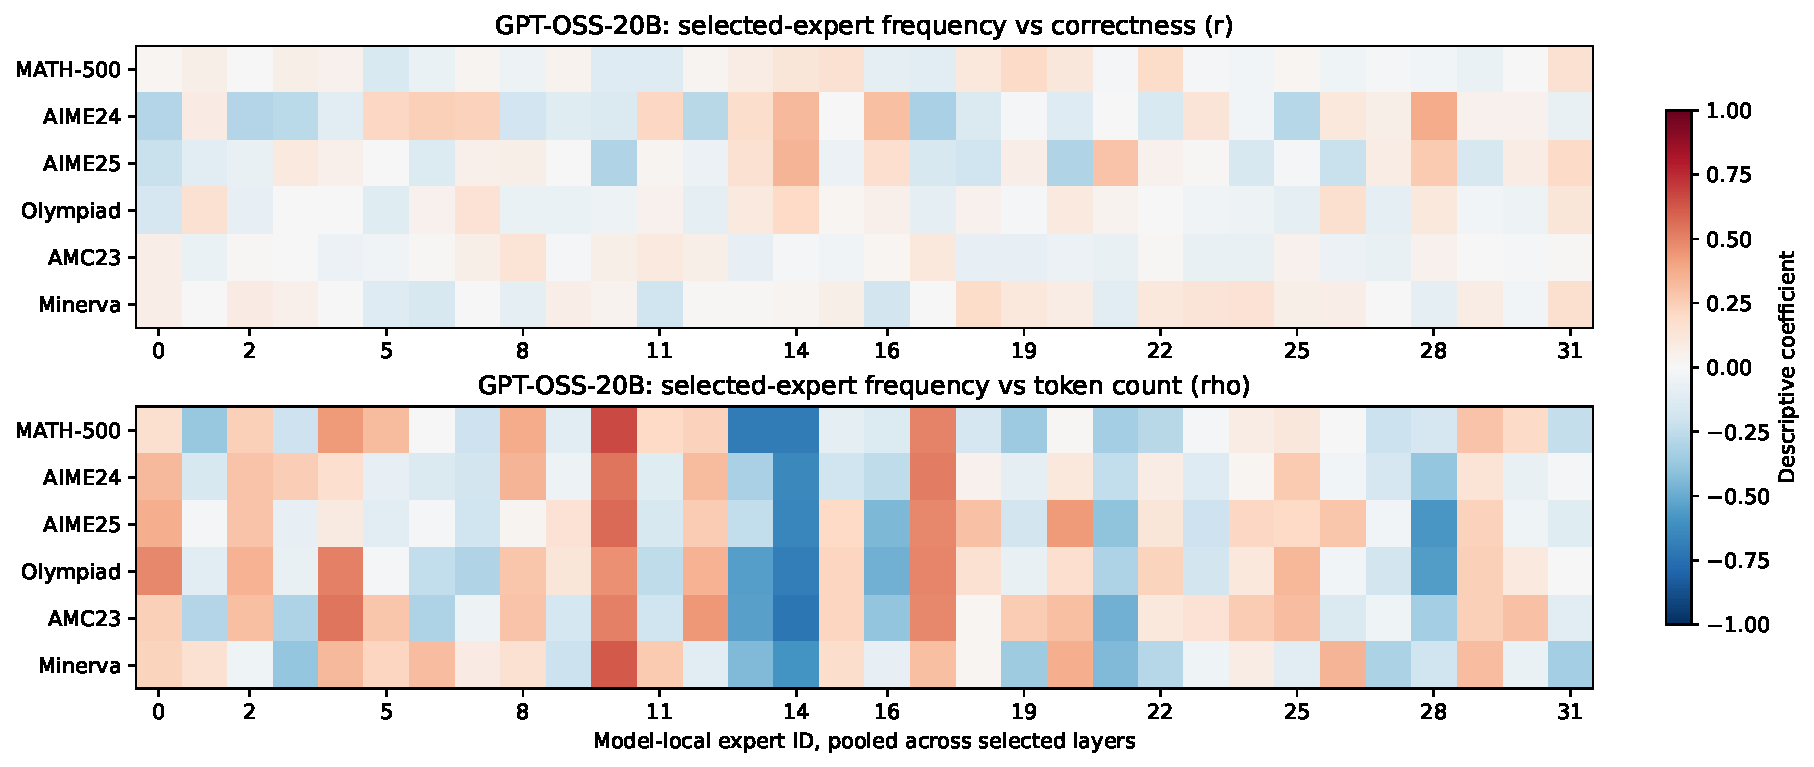
\includegraphics[width=\linewidth]{figures/gptoss_multimodel_experts.pdf}
\caption{GPT-OSS-20B: selected-pool expert frequency correlations with correctness and token count. IDs are model-local and pooled across selected layers; they do not identify matching experts across models. Missing coefficients are blank.}
\Description{GPT-OSS-20B: selected-pool expert frequency correlations with correctness and token count. IDs are model-local and pooled across selected layers; they do not identify matching experts across models. Missing coefficients are blank.}
\end{figure}


